\documentclass[border = 120pt]{standalone}

\usepackage[landscape]{geometry}
\usepackage{tikz}
\usetikzlibrary{shapes,snakes}
\begin{document}
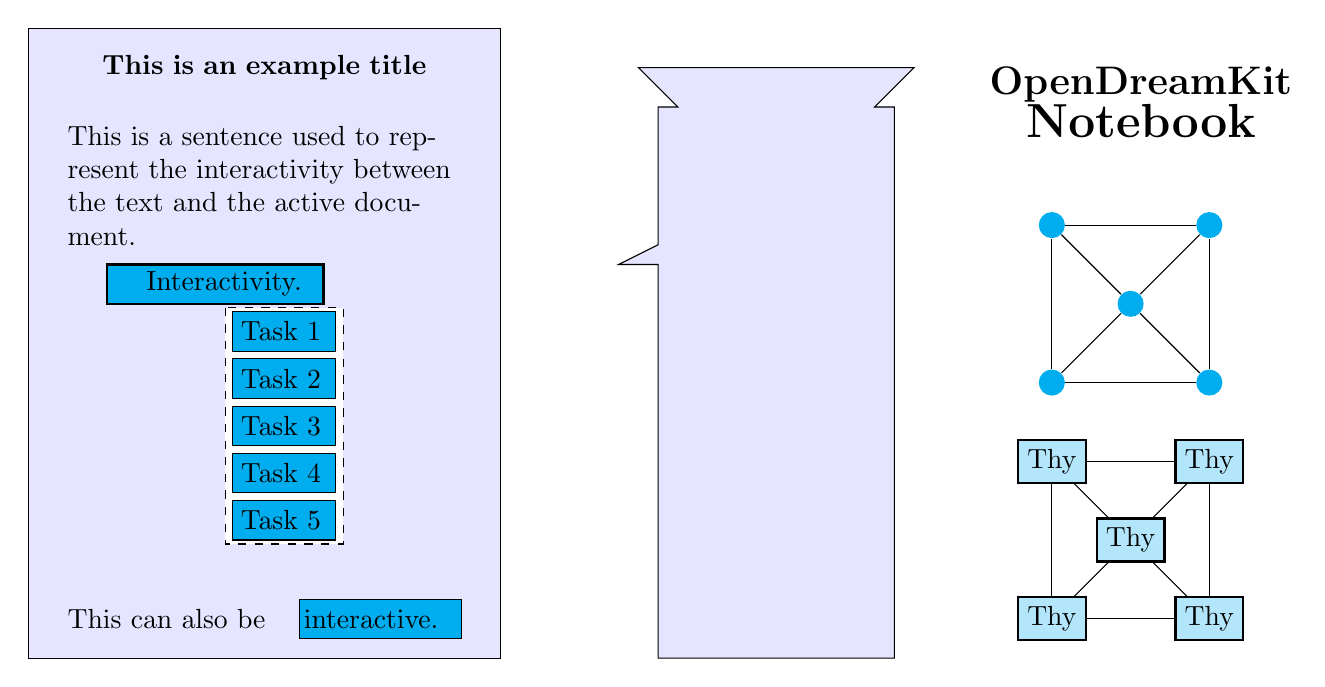
\begin{tikzpicture}

%Mother Ship
\draw[fill=blue!10] (-9,-3.5) rectangle (-15, 4.5);

%Active Document
\node[align=center, text width=5cm] at (-12,4) {\textbf{This is an example title}};
\node[align=left, text width=5cm] at (-12,2.5) {This is a sentence used to represent the interactivity between the text and the active document.};

%%Text
\draw[style=thick, fill=cyan] (-14, 1.5) rectangle (-11.25, 1);
\node[align=left, text width=5cm] at (-11,1.25) {Interactivity.};

\draw[style=dashed, fill=white] (-12.5, 0.95) rectangle (-11, -2.05);
\draw[fill=cyan] (-12.4, 0.9) rectangle (-11.1, 0.4);
\node[align=left, text width=2cm] at (-11.3,0.65) {Task 1};
\draw[fill=cyan] (-12.4, 0.3) rectangle (-11.1, -0.2);
\node[align=left, text width=2cm] at (-11.3, 0.05) {Task 2};
\draw[fill=cyan] (-12.4, -0.3) rectangle (-11.1, -0.8);
\node[align=left, text width=2cm] at (-11.3,-0.55) {Task 3};
\draw[fill=cyan] (-12.4, -0.9) rectangle (-11.1, -1.4);
\node[align=left, text width=2cm] at (-11.3,-1.15) {Task 4};
\draw[fill=cyan] (-12.4, -1.5) rectangle (-11.1, -2);
\node[align=left, text width=2cm] at (-11.3,-1.75) {Task 5};

\node[align=left, text width=5cm] at (-12,-3) {This can also be };
\draw[fill=cyan] (-11.55, -3.25) rectangle (-9.5, -2.75);
\node[align=left, text width=2cm] at (-10.5,-3) {interactive.};

% First machine
\path[draw, fill=blue!10] 
(-7, -3.5) -- 
(-7, 1.5) -- 
(-7.5, 1.5) -- 
(-7, 1.75) -- 
(-7, 3.5) -- 
(-6.75, 3.5) -- 
(-7.25, 4) -- 
(-3.75, 4) --
(-4.25, 3.5) -- 
(-4, 3.5) -- 
(-4, -3.5) -- 
cycle;


%% Jupyter Program

\node[align=center, text width=4cm] at (-1,3.5) {\textbf{\begin{tabular}{c}\Large OpenDreamKit\\\LARGE Notebook\end{tabular}}};

\node[circle,fill=cyan] (a) at (-2, 0) { };
\node[circle,fill=cyan] (b) at (0, 0) { };
\node[circle,fill=cyan] (c) at (0, 2) { };
\node[circle,fill=cyan] (d) at (-2,2) { };
\node[circle,fill=cyan] (e) at (-1, 1) { };
\foreach \from/\to in {a/b, b/c, c/d, a/d, a/e, e/b, c/e, d/e}
\draw [-] (\from) -- (\to);

\node[draw, fill=cyan!30, thick] (a) at (-2, -3) {Thy};
\node[draw, fill=cyan!30, thick] (b) at (0, -3) {Thy};
\node[draw, fill=cyan!30, thick] (c) at (0, -1) {Thy};
\node[draw, fill=cyan!30, thick] (d) at (-2, -1) {Thy};
\node[draw, fill=cyan!30, thick] (e) at (-1, -2) {Thy};
\foreach \from/\to in {a/b, b/c, c/d, a/d, a/e, e/b, c/e, d/e}
\draw [-] (\from) -- (\to);
\end{tikzpicture}
\end{document}


%%% Local Variables:
%%% mode: latex
%%% TeX-master: t
%%% End:
